	\documentclass{beamer}
	\usepackage[latin1]{inputenc}
	\usepackage{textpos}
	\usepackage{graphics}
	\usepackage[english]{babel}
	\usepackage{colortbl}
	\usepackage{caption}
	% \usepackage{subcaption}
	\usepackage{multirow}
	\usepackage{amsmath}
	\usepackage{xcolor} % for colored text

	\usepackage{tikz} % for flow charts
	\usetikzlibrary{shapes,arrows,positioning,shadows,calc}

\usepackage{filecontents}% http://ctan.org/pkg/filecontents
\usepackage{silence}% http://ctan.org/pkg/silence
\WarningFilter{latex}{Overwriting file}% Remove LaTeX warnings starting with "Overwriting file"
\begin{filecontents*}{linereg.data}
#x y
0 4
10 24
\end{filecontents*} 

\begin{filecontents*}{linereg2.data}
#x y
2 8
8 20
\end{filecontents*} 

	\renewcommand<>{\item}[1]{\only#2{\beameroriginal{\item}{#1}}} % for replace a equation for other equation in the same place
	
	% \usetheme{Warsaw}
	\usetheme{Frankfurt}
	% \usetheme{Boadilla}
	\setbeamertemplate{navigation symbols}{} 
	% \useoutertheme{infolines} 
\setbeamertemplate{footline}{\hbox{\vspace{0.1cm} \insertshortauthor \hspace*{3.5cm} \insertshorttitle \hspace*{4.6cm} \hfill\insertframenumber}} 

\def\braces#1{[#1]} % to define square parenthesis 
	
% \usecolortheme{orchid}

% \usecolortheme{lily}

% \usecolortheme{default}
\usecolortheme{cranejavier}

% \setbeamertemplate{footline}[frame number]
% \setbeamertemplate{footline}[page number]

% My packages
% added on 08-03-15
% http://www-ljk.imag.fr/membres/Jerome.Lelong/latex/appendixnumberbeamer.sty
% Reference: http://tex.stackexchange.com/questions/2541/beamer-frame-numbering-in-appendix
\usepackage{appendixnumberbeamer}
% Add total frame count to slides, optional. From Stefan,
% http://www.latex-community.org/forum/viewtopic.php?f=4&t=2173
\expandafter\def\expandafter\insertshorttitle\expandafter{%
  \insertshorttitle\hfill\insertframenumber\,/\,\inserttotalframenumber}	
	
% -------------------------------------- Slide 1 -----------------
	\title[Atmospheric Correction L8]{Atmospheric Correction for Landsat 8 over Case 2 Waters}
	\author[Javier A. Concha]{\Large Javier A. Concha, John Schott\\\vspace{1cm}}
	\institute{\footnotesize Digital Imaging and Remote Sensing Lab\\Chester F. Carlson Center for Imaging Science\\ Rochester Institute of Technology}
	\date{\today}

\AtBeginSection[ ]
{	\setbeamertemplate{footline}{} 	
	\begin{frame}{\LARGE Outline} 
	\LARGE
		\tableofcontents[currentsection]
	\end{frame}

\addtocounter{framenumber}{-1}	

\setbeamertemplate{footline}{\hbox{\vspace{0.1cm} \insertshortauthor \hspace*{3.5cm} \insertshorttitle \hspace*{4.6cm} \hfill\insertframenumber}} 
}	

% \AtBeginSubsection[ ]
% {		
% 	\begin{frame}{\LARGE Outline} 
% 		\tableofcontents[currentsection,currentsubsection]
% 	\end{frame}
% \addtocounter{framenumber}{-1}	
% }		
\newcounter{tmpc} % for resume counter
%&&&&&&&&&&&&&&&&&&&&&&&&&&&&&&&&&&&&&&&&&&&&&&&&&&&&&&&&&&&&&&&
%&&&&&&&&&&&&&&&&&&&&&&&&&&&&&&&&&&&&&&&&&&&&&&&&&&&&&&&&&&&&&&&	
	
\begin{document}
{	
\setbeamertemplate{footline}{} 
\setbeamertemplate{headline}{}
	
	\begin{frame} 
	\titlepage
	
	\begin{textblock*}{10cm}(10.0cm,-8.5cm)
	   \includegraphics[height=10mm]{/Users/javier/Desktop/Javier/MASTER_RIT/2011_THESIS/LaTeX/Presentation/tiger_walking_rit_color.eps}
	\end{textblock*}
	\begin{textblock*}{10cm}(4.7cm,-8.0cm)
	   \includegraphics[height=5mm]{/Users/javier/Desktop/Javier/PHD_RIT/ConferencesAndApplications/2014_RITResearchSymposium/Images/USGS_logo.eps}
	\end{textblock*}	
	\begin{textblock*}{10cm}(-.7cm,-8.5cm)
	   \includegraphics[height=10mm]{/Users/javier/Desktop/Javier/PHD_RIT/ConferencesAndApplications/2014_ASPRS_SOY/Images/dirs_logo.png}
	\end{textblock*}
	
	\begin{textblock*}{9cm}(2cm,-5cm)

	   \tikz\node[opacity=0.3]{ \includegraphics[width=65mm]{/Users/javier/Desktop/Javier/PHD_RIT/ConferencesAndApplications/2014_ASPRS_SOY/Images/landsat8-earth.jpg}};
	\end{textblock*}

	\begin{textblock*}{12cm}(3.7cm,0cm)
	   \scriptsize Presented to: DIRS Meeting
	\end{textblock*}
	
	\end{frame}

}
\addtocounter{framenumber}{-1}
%\setbeamercovered{highly dynamic}
%\setbeamercovered{transparent}
\setbeamercovered{still covered={\opaqueness<1->{2}},again covered={\opaqueness<1->{2}}}

% ----------------------------------- Slide ----------------------------------------------	

\addtobeamertemplate{frametitle}{}{%
\begin{textblock*}{90mm}(8.2cm,-0.5cm)
% \includegraphics[height=0.5cm]{/Users/javier/Desktop/Javier/MASTER_RIT/SPIE2012/Slides/rit_white_no_bar.jpg}
\includegraphics[height=0.4cm]{/Users/javier/Desktop/Javier/PHD_RIT/ConferencesAndApplications/2014_ASPRS_SOY/Images/RIT_LOGO.png}
\end{textblock*}}
% ----------------------------------- Slide ----------------------------------------------	
\begin{frame}{\LARGE Motivation} 
\vspace{-.5cm}
\begin{columns}[c] % contents are top vertically aligned
  	\begin{column}[T]{6cm} % each column can also be its own environment
  		\vspace{0.5cm}
      	\begin{itemize}
      	\Large
      		\item Ocean Color Satellites (e.g. MODIS, SeaWiFS): \\ \LARGE Global Studies
      	\end{itemize}
	\end{column}

  	\begin{column}[T]{6cm} % each column can also be its own environment
 		\begin{figure}[H]
 			\includegraphics[height=3cm]{/Users/javier/Desktop/Javier/PHD_RIT/ConferencesAndApplications/2014_ASPRS_SOY/Images/107325main_chloro_concentrate.jpg}
 		\end{figure}
 		\vspace{-0.7cm}
 		{\hspace{4.2cm}\tiny $*~$Credit: NASA}
 	\end{column}
\end{columns}

\begin{figure}[H]
		\includegraphics[height=4cm]{/Users/javier/Desktop/Javier/PHD_RIT/ConferencesAndApplications/2014_ASPRS_SOY/Images/DiffResol.png}
\end{figure}
\end{frame}
% ----------------------------------- Slide ----------------------------------------------
{
\setbeamertemplate{footline}{} 
\begin{frame}{\LARGE Outline} 
\LARGE
	\tableofcontents
\end{frame}

\addtocounter{framenumber}{-1}
}

%%%%%%%%%%%%%%%%%%%%%%%%%%%%%%%%%%%%%%%%%%%%%%%%%%%%%%%%%%%%%%%%%%%%%%%%%%%%%%%%%%%%%%%%%%
\section{Goal}
\subsection*{Goal}
% ----------------------------------- Slide ----------------------------------------------
\begin{frame}{\LARGE Goal} 
\begin{itemize}
\LARGE

\item To Use Landsat 8 to retrieve Color Producing Agents (CPAs):
\begin{itemize}
	\Large
 	\item chlorophyll
 	\item colored dissolved organic matter (CDOM)
 	\item suspended minerals (SM or TSS)
 \end{itemize}
\vspace{.5cm}
\item Over Coastal and Inland Water (Case 2 Waters)
\vspace{.5cm}
\item Small/Medium Scale regions

\end{itemize}

\end{frame}

%%%%%%%%%%%%%%%%%%%%%%%%%%%%%%%%%%%%%%%%%%%%%%%%%%%%%%%%%%%%%%%%%%%%%%%%%%%%%%%%%%%%%%%%%%
\section{Background}
% ------------------------------ SUBSECTION ----------------------------------------------
\subsection*{Atmospheric Correction: ELM}
% ----------------------------------- Slide ----------------------------------------------
\begin{frame}{\LARGE Atmospheric Correction} 
 \begin{columns}[c] % contents are top vertically aligned
  	\begin{column}[T]{5cm} % each column can also be its own environment
    \includegraphics[height=5cm]{/Users/javier/Desktop/Javier/PHD_RIT/ConferencesAndApplications/2014_RITResearchSymposium/Images/SensorReachingRadiance.png}
    	    \vspace{0.2cm}
    		\centerline{Retrieve $L_w$}
     	\end{column}
  
  	\begin{column}[T]{7cm} % each column can also be its own environment
    \includegraphics[width=7cm]{/Users/javier/Desktop/Javier/PHD_RIT/ConferencesAndApplications/2014_RITResearchSymposium/Images/TOARadiance.png}
    	    \vspace{0.2cm}
    		\centerline{Retrieve $L_w$ vs $L_u$}
    		% \centerline{(Unknown concentrations)}
     	\end{column}
\end{columns}
\vspace{.5cm}
\hspace{4cm}{\scriptsize $*~$Images from: http://www.oceanopticsbook.info/}
\end{frame}
% ----------------------------------- Slide ----------------------------------------------
\begin{frame}{\LARGE Atmospheric Correction}
{\Large Empirical Line Method (ELM)} 
 \begin{columns}[c] % contents are top vertically aligned
  	\begin{column}[T]{5cm} % each column can also be its own environment
  	{\centering \Large $L(\lambda)=m\times R_{rs}(\lambda)+b$}\\
  	\vspace{0.1cm}
  	where: \begin{tabbing} $L$: Radiance\\
  	$R_{rs}=\frac{Lw}{E_d}$: Remote-sensing\\ ~~~~~~~~~~~~~~~~~~reflectance\\
  	$m$: slope\\
  	$b$: offset
  	\end{tabbing}
  	% \vspace{0.3cm}
    \begin{itemize}
    	\item Two pixels in the scene with known reflectance
    	\vspace{0.3cm}
    	% \item Linear relationship between radiance $L$ and reflectance $r_d$ 	
    \end{itemize}
     	\end{column}
  
  	\begin{column}[T]{7cm} % each column can also be its own environment
	\centering
\begin{figure}[htb]
	\centering
\resizebox{7cm}{!}{%
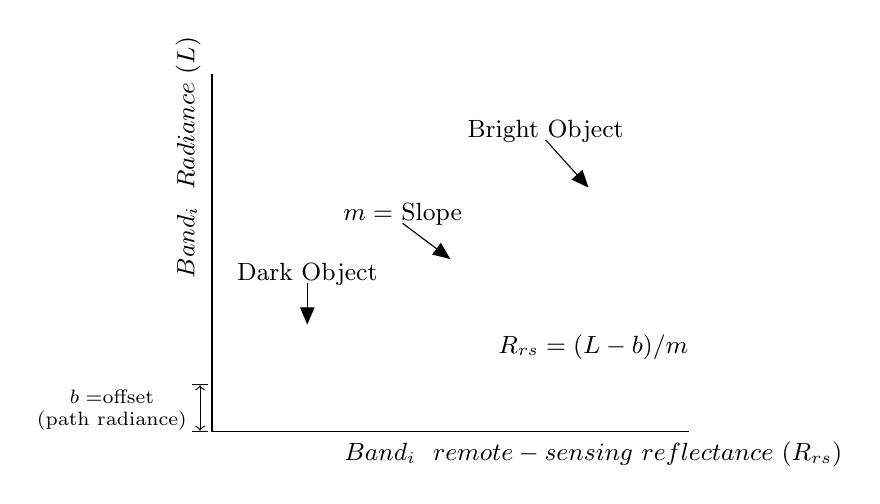
\begin{tikzpicture}[x=4ex,y=1ex]
 	%axis
	\draw (0,0) -- coordinate (x axis mid) (10,0);
    \draw (0,0) -- coordinate (y axis mid) (0,30);
 
    %labels      
	\node[below=0ex] at (8,0) {\small $Band_i~~remote-sensing~reflectance~(R_{rs})$};
	\node[rotate=90] at (-.5,23) {\small $Band_i~~Radiance~(L)$};

	\node[below=.2ex] at (-2.1,4.5) {\scriptsize $b=$offset};
	\node[below=1.4ex] at (-2.1,4.0) {\scriptsize (path radiance)};
	\draw[rotate=90,|<->|] (0,1) -- coordinate (x axis mid) (1,1);

	\node[below=0ex] at (2,15) {\small Dark Object};
	\draw[arrows=-triangle 45] (2,12.5) -- (2,9);

	\node[below=0ex] at (4,20) {\small $m=$ Slope};
	\draw[arrows=-triangle 45] (4,17.5) -- (5,14.5);

	\node[below=0ex] at (7,27) {\small Bright Object};
	\draw[arrows=-triangle 45] (7,24.5) -- (7.9,20.5);

	\node[below=0ex] at (8,9) {\small $R_{rs}=(L-b)/m$};

	%plots
	\draw plot 
		file {linereg.data};
	\draw plot[mark=*] 
		file {linereg2.data};

\end{tikzpicture}
% \caption{MoB-ELM atmospheric correction method. The MoB-ELM method is based on the traditional empirical line method (ELM). Two pixels from the image, the bright and dark pixel, are used to solve a liner regression with a slope $m$ and offset $b$ in the $R_{rs}$, $L$ space. Once this relationship is established, each $L$ value in the image can be converted to $R_{rs}$ through $R_{rs}=(L-b)/m$. \label{fig:ELMregression}
} % end resize
\end{figure}

     	\end{column}
\end{columns}

\end{frame}% ------------------------------ SUBSECTION ----------------------------------------------
\subsection*{Landsat 8}
% ----------------------------------- Slide ----------------------------------------------
\begin{frame}{\LARGE Landsat 8 - OLI Specifications} 
\vspace{-.5cm}
\begin{itemize}
\LARGE
	\item Optical satellite (passive)
	\vspace{.2cm}
	\item Multispectral: 4 VIS, 1 NIR, 2 SWIR, 1 Pan
	\vspace{.2cm}
	\item Spatial resolution: 15/30/100m
	\vspace{.2cm}
	\item Temporal resolution: 16 days
	\vspace{.2cm}
	\item Bit depth: 12-bits quantization (4096 levels)
	\vspace{.2cm}
	\item Pushbroom satellite
\end{itemize}

\end{frame}
% % ----------------------------------- Slide ----------------------------------------------
% \begin{frame}{\LARGE Landsat 8} 

% \begin{figure}[H]
% 		\includegraphics[height=6cm]{/Users/javier/Desktop/Javier/PHD_RIT/ConferencesAndApplications/2014_ASPRS_SOY/Images/ldcmbands.png}
% \end{figure}

% \end{frame}
% ----------------------------------- Slide ----------------------------------------------
\begin{frame}{\LARGE Landsat 8 Image} 
\begin{figure}[htb]
  	\centering
  	\includegraphics[height=7cm]{/Users/javier/Desktop/Javier/PHD_RIT/Latex/Proposal/Images/LC80160302013262LGN00subset.jpg}
  % \caption{Portion of the Landsat 8 image to be corrected showing part of the Lake Ontario, nearby ponds and Downtown Rochester. \label{fig:Scene} } 
\end{figure}
\end{frame}
% ----------------------------------- Slide ----------------------------------------------
% ------------------------------ SUBSECTION ----------------------------------------------
\subsection*{Physics Model: Hydrolight}
\begin{frame}{\LARGE Hydrolight} 
\centerline{\LARGE For the Dark Pixel and LUT generation}

\begin{figure}[H]
		\includegraphics[height=6cm]{/Users/javier/Desktop/Javier/PHD_RIT/ConferencesAndApplications/2014_ASPRS_SOY/Images/HLdiagram.pdf}
\end{figure}
\hspace{5cm}{$*~$IOPs: Inherent Optical Properties}
\end{frame}
%%%%%%%%%%%%%%%%%%%%%%%%%%%%%%%%%%%%%%%%%%%%%%%%%%%%%%%%%%%%%%%%%%%%%%%%%%%%%%%%%%%%%%%%%%
\section{Atmospheric Correction}
\subsection*{}
% ----------------------------------- Slide ----------------------------------------------
\begin{frame}{\LARGE Atmospheric Correction} 
{\Large Model-Based ELM}

\begin{block}{\LARGE Bright Pixel}
 	\begin{itemize}
 	\Large
 		\item Radiance: PIF\footnotemark[1] from Landsat 8 image
 		\item Reflectance: PIF\footnotemark[1] from Landsat reflectance product
 	\end{itemize}
\end{block} 
% \vspace{0.1cm}
\begin{block}{\LARGE Dark Pixel}

	\begin{itemize}
	\Large
		\item Radiance: ROI\footnotemark[2] over water from Landsat 8 image
		\item Reflectance: Hydrolight
	\end{itemize}

\end{block}
\footnotetext[1]{Pseudo-Invariant Features}
\footnotetext[2]{Region of interest}

\end{frame}
% ----------------------------------- Slide ----------------------------------------------
\begin{frame}{\LARGE Atmospheric Correction} 
{\Large Pseudo-Invariant Features -- Bright Pixel}

\begin{figure}[htb]
  \begin{minipage}[c]{0.48\linewidth}
    \centering
      \includegraphics[trim=30 0 30 0,clip,height=5cm]{/Users/javier/Desktop/Javier/PHD_RIT/Latex/Proposal/Images/DTROCL8falsecolor.jpg}  
    \vspace{0.3cm}
    \centerline{Downtown Rochester}
    \centerline{False Color Image}
  \end{minipage}
  \hfill
  \begin{minipage}[d]{0.48\linewidth}
    \centering
      \includegraphics[trim=30 0 30 0,clip,height=5cm]{/Users/javier/Desktop/Javier/PHD_RIT/Latex/Proposal/Images/PIFmaskApplied.jpg}
    \vspace{0.3cm}
    \centerline{Downtown Rochester}
    \centerline{PIF mask}
  \end{minipage}
  % \caption{PIF mask determination. (a) False color image, with vegetation in red and (b) PIF mask over downtown Rochester. \label{fig:PIFmask} } 
\end{figure}
\end{frame}

% % ----------------------------------- Slide ----------------------------------------------
% \begin{frame}{\LARGE Atmospheric Correction} 
% {\Large PIFs -- Bright Pixel}

% \begin{figure}[htb]
%   \begin{minipage}[c]{0.48\linewidth}
%     \centering
%       \includegraphics[height=4.8cm]{/Users/javier/Desktop/Javier/PHD_RIT/Latex/Proposal/Images/ZenithCorrection.eps}
%   % \caption{Mean values for nine scenes of the Landsat reflectance product after applying the master PIF mask. \label{fig:ZenithCorr} }   
%     \vspace{0.3cm}
%     \centerline{PIFs values for 9}
%     \centerline{Landsat reflectance images}
%   \end{minipage}
%   \hfill
%   \begin{minipage}[d]{0.48\linewidth}
%     \centering
%       \includegraphics[height=4.8cm]{/Users/javier/Desktop/Javier/PHD_RIT/Latex/Proposal/Images/ZenithCorrelation.eps}
%   % \caption{Linear regression between reflectance values and solar zenith angle for band 1 of the Landsat reflectance product. \label{fig:Band1Corr} }
%     \vspace{0.3cm}
%     \centerline{Band 1 - PIFs spectrum for 9}
%     \centerline{Landsat reflectance images}
%   \end{minipage}
%   % \caption{PIF mask determination. (a) False color image, with vegetation in red and (b) PIF mask over downtown Rochester. \label{fig:PIFmask} } 
% \end{figure}
% \end{frame}
% ----------------------------------- Slide ----------------------------------------------
\begin{frame}{\LARGE Atmospheric Correction} 
{\Large Dark Pixel}

\begin{columns}[c] % contents are top vertically aligned
  	\begin{column}[T]{6cm} % each column can also be its own environment

		\includegraphics[height=4cm]{/Users/javier/Desktop/Javier/PHD_RIT/ConferencesAndApplications/2014_RITResearchSymposium/Images/StudyArea.png}
	\end{column}

  	\begin{column}[T]{6cm} % each column can also be its own environment
  		\begin{itemize}
  			\item Radiance: Lake Ontario ROI
  			\vspace{.5cm}
  			\item Reflectance: Hydrolight with IOPs measured in the field over same ROI
  		\end{itemize}
 	\end{column}
\end{columns}

\end{frame}
% ----------------------------------- Slide ----------------------------------------------
\begin{frame}{\LARGE Atmospheric Correction} 
{\Large Model-Based ELM}
\centerline{\LARGE Bright and Dark Pixel}

\begin{figure}[htb]
  \begin{minipage}[c]{0.48\linewidth}
    \centering
      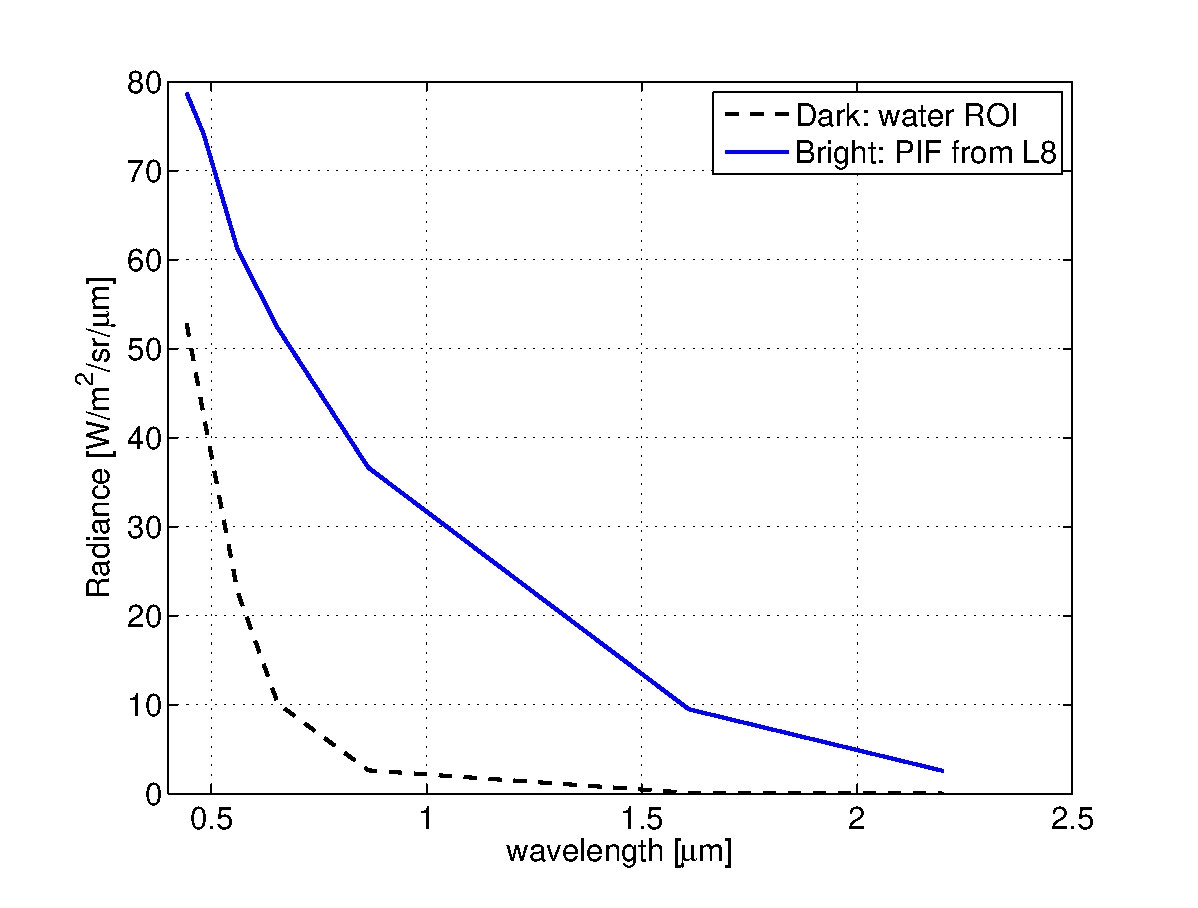
\includegraphics[width=6cm]{./Images/ELMrad130929_150422}
    \vspace{0.3cm}
    \centerline{(a) Radiance}\medskip
  \end{minipage}
  \hfill
  \begin{minipage}[d]{0.48\linewidth}
    \centering
      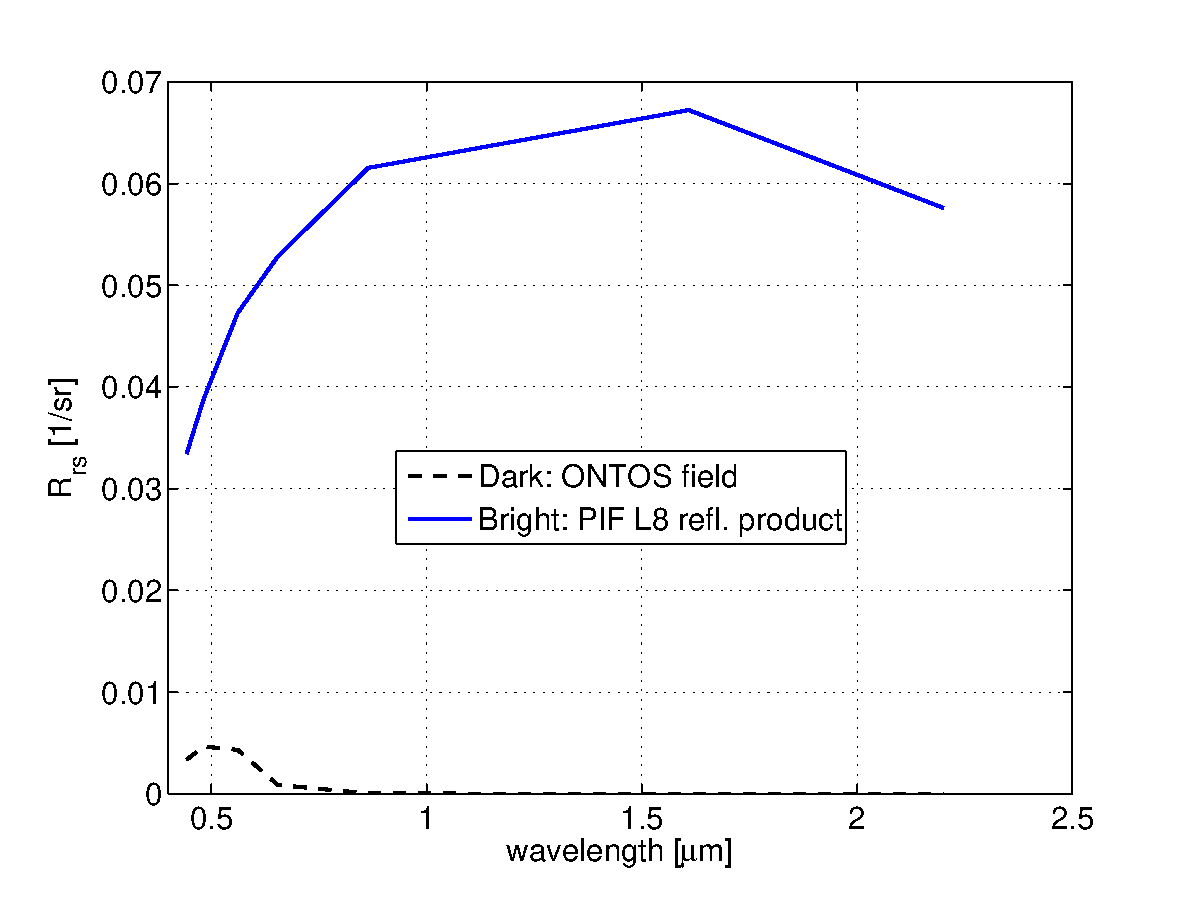
\includegraphics[width=6cm]{./Images/ELMRrs130929_150422}
    \vspace{0.3cm}
    \centerline{(b) $R_{rs}$}\medskip
  \end{minipage}
  % \caption{Example of the bright and dark pixel used in the MoB-ELM atmospheric correction method for Landsat 8 scene acquired on 09-19-2013.\label{fig:MOBELMpxls} } 
\end{figure}

\end{frame}

%%%%%%%%%%%%%%%%%%%%%%%%%%%%%%%%%%%%%%%%%%%%%%%%%%%%%%%%%%%%%%%%%%%%%%%%%%%%%%%%%%%%%%%%%%
\section[Chl-{\it a} Retrieval]{Chlorophyll-{\it} Retrieval}
\subsection*{}
% ----------------------------------- Slide ----------------------------------------------
\begin{frame}{\LARGE Chlorophyll-{\it a} Retrieval Process} 

\begin{figure}[H]
		\includegraphics[height=7cm]{/Users/javier/Desktop/Javier/PHD_RIT/ConferencesAndApplications/2014_ASPRS_SOY/Images/RetProcess.pdf}
\end{figure}

\end{frame}
% ----------------------------------- Slide ----------------------------------------------

\begin{frame}{\LARGE Retrieval} 
{\vspace{0.1cm} \Large LUT from Hydrolight}
% \begin{block}{\footnotesize LUT}
  \begin{columns}[c] % contents are top vertically aligned
  	\begin{column}[T]{6cm} % each column can also be its own environment
  	\vspace{0.2cm}
    	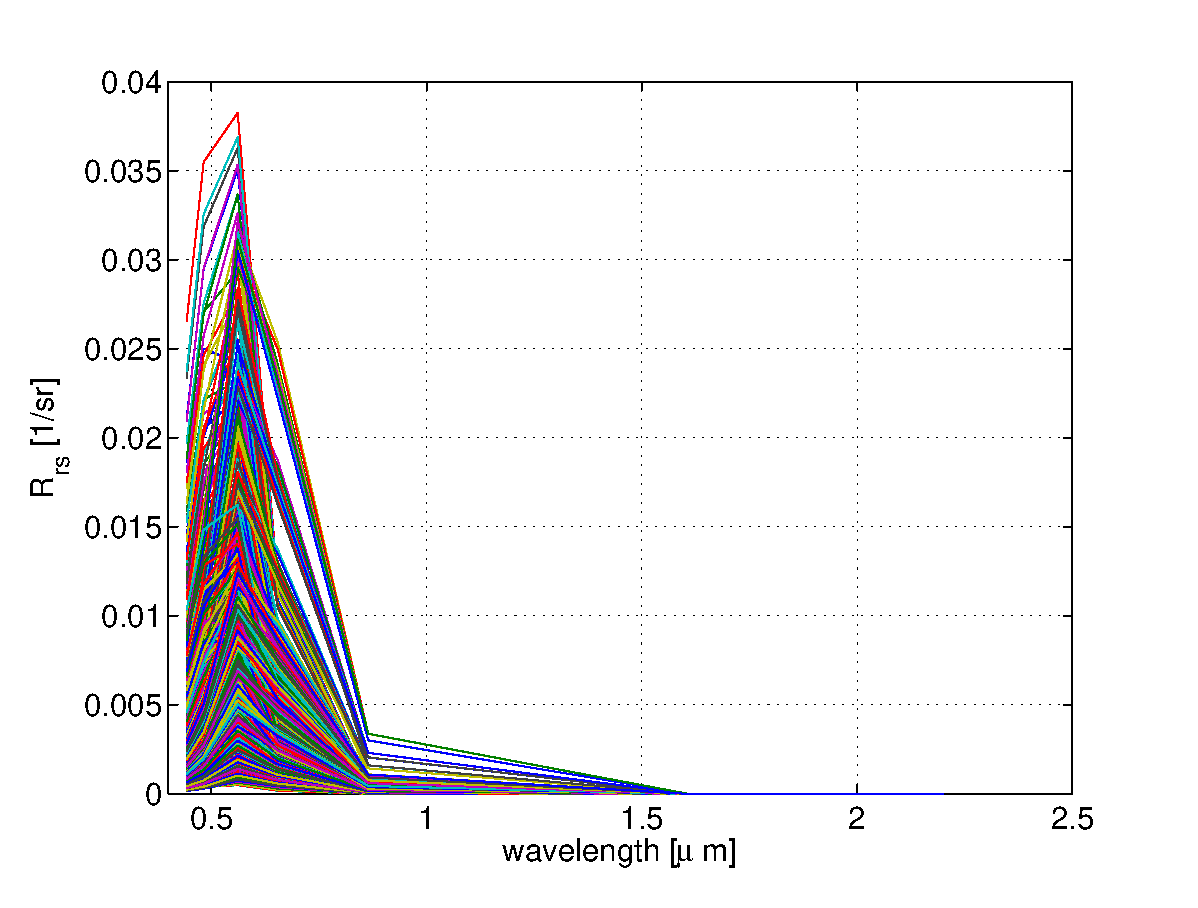
\includegraphics[height=5cm]{/Users/javier/Desktop/Javier/PHD_RIT/ConferencesAndApplications/2015_Landsat_Special_Issue/Images/LUTsmart130919_150422.eps}
    	    \vspace{0.2cm}
    		\centerline{LUT}
    		\centerline{(Known concentrations)}
    \end{column}
  	\hspace{.3cm}
  	\begin{column}[T]{6cm} % each column can also be its own environment
  	\vspace{0.2cm}
	\scriptsize \addtolength{\tabcolsep}{-5pt}
\begin{table}[htb]
% \caption{Input parameters for the LUT generation in Hydrolight for the Landsat 8 image acquired on 09-19-2013. \label{tab:LUTconc}} 
\tiny
\centering
    \begin{tabular}{ccccc}
    \hline \hline
            IOPs Input & \bfseries{$C_a$} & \bfseries{$TSS$} & \bfseries{$a_{CDOM}(440nm)$} & \bfseries{$b_b/b$}    \\
                   & $[mg~m^{-3}]$        & $[g~m^{-3}]$       &  $[1/m]$           & $[\%]$            \\ \hline \hline
\multirow{8}{*}{ONTNS}  &  0.1    	& 1.0     &  0.11   &  0.3  \\
   	&  0.5    	& 2.0   &  0.15   	&  0.4  \\
    &  1.0    	& 5.0   &  0.21   	&  0.5  \\
    &  3.0    	& 10.0  &  0.6    	&  0.6  \\ 
    &  10.0     & --    &  --   	&  0.7  \\  
    &  20.0     & --    &  --   	&  1.0  \\  
    &  40.0     & --    &  --   	&  1.4  \\
    &  --       & --    &  --   	&  2.0  \\ \hline

\multirow{8}{*}{LONGS}   &  60.0   & 25.0    &  1.0    &  0.3  \\
    &  90.0   & 45.0    &  1.2    &  0.4  \\
    &  110.0  & 50.0    &  --     &  0.5  \\
    &  --     & --      &  --     &  0.6  \\  
    &  --     & --      &  --     &  0.7  \\  
    &  --     & --      &  --     &  1.0  \\   
    &  --     & --      &  --     &  1.4  \\  
    &  --     & --      &  --     &  2.0  \\  \hline \hline
% --      &  135.0  & --      &  --     &  --   \\  
% --      &  150.0  & --      &  --     &  --   \\ \hline 
    \end{tabular}
  \end{table}
     	\end{column}
\end{columns}
% \end{block}
\end{frame}

%%%%%%%%%%%%%%%%%%%%%%%%%%%%%%%%%%%%%%%%%%%%%%%%%%%%%%%%%%%%%%%%%%%%%%%%%%%%%%%%%%%%%%%%%%
\section{Conclusions}
\subsection*{Conclusions}
% ----------------------------------- Slide ----------------------------------------------
\begin{frame}{\LARGE Take Home Points} 
\begin{itemize}
\Large
\setbeamercovered{transparent}
    \uncover<2->{
	\item Landsat 8 has a great potential to help in fresh and coastal water quality studies}
	\vspace{\baselineskip}
	\uncover<3->{
	\item Atmospheric correction over water is an essential step}
	\vspace{\baselineskip}
	\uncover<4->{
	\item Hydrolight is an excellent tool BUT needs specific water characteristics}
\end{itemize}
\end{frame}
 % ----------------------------------- Slide ----------------------------------------------
% \section*{}
% \begin{frame}%[shrink=30] 
% \tiny
%   \frametitle{References}
%   \nocite{*}
%   \bibliographystyle{apalike}
%   \bibliography{HLbeamerbib}
% \end{frame}

%% ----------------------------------- Slide ----------------------------------------------

{	
\setbeamertemplate{footline}{} 
\setbeamertemplate{headline}{}
\begin{frame}[noframenumbering] 

\vspace{\baselineskip}
\centerline{\Large Thanks for your attention!}
	\vspace{\baselineskip}

% \centerline{\Huge QUESTIONS?}
\uncover <2->{\centerline{\Huge QUESTIONS?}}
\vspace{\baselineskip}
\centerline{Javier A. Concha}
\centerline{jxc4005@rit.edu}

\begin{figure}[htb]
\centering
\includegraphics[height=5cm,clip=true]{/Users/javier/Desktop/Javier/PHD_RIT/Latex/Proposal/Images/L8Glint.png}
\end{figure}

\end{frame}
}
% #################################################################################
% ########################## END PRESENTATION #####################################
% #################################################################################
\appendix
\section{Additional Material}
% ----------------------------------- Slide ----------------------------------------------
% ------------------------------ SUBSECTION ----------------------------------------------
\subsection*{Field Collection and Lab Measurements}
\begin{frame}{\LARGE Field Collection} 
\begin{figure}[htb]
  \centering
  \includegraphics[width=8cm]{/Users/javier/Desktop/Javier/PHD_RIT/Latex/Proposal/Images/groundtruth-sitenames-no-ends.jpg}
  % \caption{Sites in the Rochester Embayment for the water sample collection on September, $19^{th}$, 2013.\label{fig:0910913Sites} } 
\end{figure}
\end{frame}
% ----------------------------------- Slide ----------------------------------------------
\begin{frame}{\LARGE Field Collection (con't)} 
\vspace{-1cm}
\begin{figure}[htb]
\centering
\includegraphics[height=7cm]{/Users/javier/Desktop/Javier/PHD_RIT/ConferencesAndApplications/2014_ASPRS_SOY/Images/Collection.pdf}
      
\end{figure}
% \centerline{Comparison between traditional ELM (dashed lines)}
% \centerline{and model-based ELM (solid lines).}
\end{frame}
% ----------------------------------- Slide ----------------------------------------------
\begin{frame}{\LARGE Lab Measurements} 
\vspace{-1cm}
\begin{figure}[htb]
\centering
\includegraphics[height=7cm]{/Users/javier/Desktop/Javier/PHD_RIT/ConferencesAndApplications/2014_ASPRS_SOY/Images/LabMeasurements.pdf}
      
\end{figure}
% \centerline{Comparison between traditional ELM (dashed lines)}
% \centerline{and model-based ELM (solid lines).}
\end{frame}
\end{document} % EEEEEEEEEEENNNNNNNNNNNNNNDDDDDDDDDDDD